The models built in Section VI were used to classify the samples of spectrograms. Different approaches are used to assess the accuracies obtained with these models. This section compares the performances of these models for the different classification tasks. 
\subsection{Accuracy assessment}
We compared the performances of the classifiers using different assessment methods: \begin{enumerate*} \item overall classification accuracy (OA); \item average class accuracy (AA); \item Recall; \item F1 score.\end{enumerate*} OA is given as
\begin{equation}
OA=\frac{\sum_{i=1}^{C}n_{ii}}{n}
\end{equation}
where $C$ is the number of existing classes,  $n_{ii}$ is the number of samples of class $i$ that are classified rightly in the prediction and $n$ is the total number of labeled samples used in the prediction. OA provides the rate of correctly classified samples. However, it is biased towards the classes that have a high frequency relative to other classes. Unlike OA, Recall, AA and F1 score provide an average of measures independent of class distribution. The Recall method can be calculated by
\begin{equation}
Recall=\frac{\sum_{i=1}^{C}n_{ii}}{\sum_{i=1}^{C}n_{i+}}
\end{equation}
where $n_{i+}$ represents the number of reference samples of class $i$.

The average class accuracy can be calculated by
\begin{equation}
AA=\frac{1}{C}\sum_{i=1}^{C}\frac{n_{ii}}{n_{i+}}
\end{equation}

The F1 score can be calculated by 
\begin{equation}
F1= 2 \frac{ Precision \times Recall}{Precision+Recall}
\end{equation}
where $Precision$ is given by
\begin{equation}
Precision=\frac{\sum_{i=1}^{C}n_{ii}}{\sum_{i=1}^{C}n_{+i}}
\end{equation}
where $n_{+i}$ represents the number of samples that are  predicted to be as class $i$.

Recall provides the rate of correctly classified samples of class $i, (1 \leq i\leq C)$ within all reference samples of class $i$, while AA computes the average rate of correctly classified spectrograms within each class, and F1 calculates the harmonic mean of the precision and recall.

\subsection{The Results for Human recognition}
The aim of the human recognition is to differentiate human from other targets based on their different micro-Doppler signatures. Animals are the most common confusers. In this paper, a dog was used to represent four-legged animals. According to the type of the targets, the samples were divided into four categories (e.g. human, dog, human and dog, and background/none). The performances of CNN, SVM, and \textit{k}NN are shown in Table \ref{tb-hc}. The CNN achieved the highest performance in all different metrics, with 97.5\% in OA, 96.69\% in AA, 97.23\% in Recall, and 97.22\% in F1. It outperforms SVM+2D2PCA and \textit{k}NN+2D2PCA with 1\%-7\% in OA and AA, 0.8\%-6.2\% in Recall and F1. SVM and \textit{k}NN greatly lag behind of all the others.
\begin{table}[]
\centering
\caption{Performance in human recognition}
\label{tb-hc}
\begin{tabular}{|l|l|l|l|l|}
\hline
\textbf{MODEL} & \textbf{OA} & \textbf{AA} & \textbf{RECALL} & \textbf{F1} \\ \hline
SVM            & 74.4\%      & 72.35\%     & 75.52\%         & 74.76\%     \\ \hline
SVM+2D2PCA     & 96.5\%      & 95.69\%     & 96.4\%          & 96.4\%      \\ \hline
KNN            & 66.2\%      & 64.60\%     & 66.23\%         & 65.54\%     \\ \hline
KNN+2D2PCA     & 91.1\%      & 89.69\%     & 91.41\%         & 91.24\%     \\ \hline
CNN (RadarNet) & 97.5\%      & 96.69\%     & 97.23\%         & 97.22\%     \\ \hline
\end{tabular}
\end{table}

\subsection{Results for Human activity detection}
Two types of human activities (walking and running) were investigated in the experiments. So the `human` samples can be divided into two further classes. The performances of the classifiers are shown in Table \ref{tb-had}. The best performance of 99.89\% in OA, AA, Recall, and F1 was achieved by our RadarNet, and SVM+2D2PCA follows it closely with 99.4\% in OA, 99.33\% in AA, and 99.3\% in Recall and F1. \textit{k}NN+2D2PCA also achieved a good result of 98.35\% in OA, 98.12\% in AA, 97.2\% in Recall, and 98.2\% in F1. The above three classifiers outperform SVM and \textit{k}NN by a wide margin.
\begin{table}[]
\centering
\caption{Performance in human activity detection}
\label{tb-had}
\begin{tabular}{|l|l|l|l|l|}
\hline
\textbf{MODEL} & \textbf{OA} & \textbf{AA} & \textbf{RECALL} & \textbf{F1} \\ \hline
SVM            & 86.6\%      & 87.6\%      & 85.8\%          & 88.13\%     \\ \hline
SVM+2D2PCA     & 99.4\%      & 99.33\%     & 99.3\%          & 99.38\%     \\ \hline
KNN            & 83.3\%      & 83.16\%     & 83.16\%         & 84.3\%      \\ \hline
KNN+2D2PCA     & 98.35\%     & 98.12\%     & 97.2\%          & 98.2\%      \\ \hline
CNN (RadarNet) & 99.89\%     & 99.89\%     & 99.89\%         & 99.89\%       \\ \hline
\end{tabular}
\end{table}

\subsection{Results for People counting}
In \textit{Case 1}, the micro-Doppler signatures of a single person were collected. In \textit{Case 2}, samples for groups of two, three, and four people were collected by our radar system. So for people counting, the `human`' samples can be further divided into four classes according to the number of people. The performances of the classifiers in people counting are shown in Table \ref{tb-pc}. RadarNet still achieved the best performance results with 98.85\% in OA, 98\% in AA, 98.85\% in Recall, and 98.7\% in F1, followed by SVM+2D2PCA with 95.9\% in OA, 95.7\% in AA, and 95.9\% in Recall and F1. The performance of \textit{k}NN+2D2PCA lags behind SVM+2D2PCA with around 12.5\% in OA, AA, Recall, and F1. SVM and \textit{k}NN had very poor performances in people counting.
\begin{table}[]
\centering
\caption{Performance in people counting}
\label{tb-pc}
\begin{tabular}{|l|l|l|l|l|}
\hline
\textbf{MODEL} & \textbf{OA} & \textbf{AA} & \textbf{RECALL} & \textbf{F1} \\ \hline
SVM            & 65.3\%      & 58\%        & 65.3\%          & 63\%        \\ \hline
SVM+2D2PCA     & 95.9\%      & 95.7\%      & 95.9\%          & 95.9\%      \\ \hline
KNN            & 60.46\%     & 52.6\%      & 61\%            & 58.4\%      \\ \hline
KNN+2D2PCA     & 83.3\%      & 83.4\%      & 81.88\%         & 83.4\%      \\ \hline
CNN (RadarNet) & 98.85\%     & 98\%        & 98.85\%         & 98.7\%      \\ \hline
\end{tabular}
\end{table}

\subsection{Results for Coarse-grained localization of human targets}
In the experiments, the detection area was split into three non-overlapping ranges, which were 1-3m, 3-5m, and 5-7m relative to the primary node. The coarse-grained localization estimates which range the location of the human target belongs to. With these three ranges, the samples of the human target were divided into three categories. The performances of the classifiers for coarse-grained localization are shown in Table \ref{tb-loc}. The overall performance achieved in coarse-localization is higher than other three classification tasks. The CNN perfectly estimated the range where the target was located in. SVM+2D2PCA presented slight inferior results, with 99.9\% in OA, and 99.87\% in AA, Recall, and F1. \textit{k}NN+2D2PCA also performed very well with the lowest accuracy metric achieving 99.19\%. SVM underperformed SVM+2D2PCA by around 12\% in the different accuracy metrics, with around 88\% in OA, Recall and F1, and 87.25\% in AA. Finally, \textit{k}NN presented the lowest scores, achieving a percentage of around 81\% in the different metrics.
\begin{table}[]
\centering
\caption{Performance in Coarse-grained localization}
\label{tb-loc}
\begin{tabular}{|l|l|l|l|l|}
\hline
\textbf{MODEL} & \textbf{OA} & \textbf{AA} & \textbf{RECALL} & \textbf{F1} \\ \hline
SVM            & 88.2\%      & 87.25\%     & 88\%            & 88\%        \\ \hline
SVM+2D2PCA     & 99.9\%      & 99.87\%     & 99.87\%         & 99.87\%     \\ \hline
KNN            & 81.8\%      & 81.42\%     & 81.08\%         & 81\%        \\ \hline
KNN+2D2PCA     & 99.19\%     & 99.24\%     & 99.19\%         & 99.19\%     \\ \hline
CNN (RadarNet) & 100\%       & 100\%       & 100\%           & 100\%       \\ \hline
\end{tabular}
\end{table}

\subsection{Analysis}
Based on the above results achieved by the classifiers in four different classification tasks, the chart presented in Fig. \ref{fig_rsu} was plotted. It is clear from the chart that, in all four tasks, the highest performance (OA) of the classifiers is given by the CNN (RadarNet), followed by the SVM+2D2PCA, then \textit{k}NN+2D2PCA. The classifiers with lower accuracy results were SVM and \textit{k}NN. As one of the most popular deep learning algorithms, CNN proved to be very suitable for micro-Doppler signature-based classification. CNN achieved the best OA scores, which were 97.5\% in human recognition, 99.89\% in human activity detection, 98.85\% in people counting, and 100\% in coarse-grained localization. SVM+2D2PCA follows closely and \textit{k}NN+2D2PCA is slightly inferior to SVM+2D2PCA, but both of them exceeded SVM and \textit{k}NN by a wide margin between 11\%-18\%. The performances of SVM and \textit{k}NN were greatly improved by the features extraction using 2D2PCA.   

From the aspect of classification tasks, different classification tasks have different levels of difficulty, which indicates whether samples in a classification task are easier or more difficult to be classified. If the tasks are sorted by order of difficulty, the order would be: $People\;  Counting> Human\;  Recognition>Human\;  Activity\;  Detection>Rough\;  localization$. This can be seen in Fig. \ref{fig_rsu}, the average performance of all classifiers for coarse-grained localization is the highest compared to the average performance of the other classification tasks, followed by the average for human detection and human recognition. While the average accuracy results for people counting are the lowest of all. Fig. \ref{fig_confusion} shows the \textit{confusion matrices} of CNNs for the four classification tasks. A \textit{confusion maxtrix} is a table used to describe the performance of a classification model (or `‘classifier`’) on a set of test data for which the true values are known. All correct predictions are located in the diagonal of the table. It allows the visualization of the performance of a classifier. In Fig. \ref{fig_confusion}(a), the most misclassified samples were from the `‘Human and Dog`’, and they were classified into `‘Human`’. This implies that it is relatively difficult to differentiate the micro-Doppler signatures of these two classes. In Fig. \ref{fig_confusion}(b), six samples of `‘Walking`’ were classified into `‘Running`’, this could be probably because different participants have different walking speeds, and fast-walking people and slow-running people generated more similar micro-Doppler signatures that is harder to differentiate. Fig. \ref{fig_confusion}(c) presents 12 out 13 misclassified samples of `‘1 person`’ that were classified into `‘2 people`’; 13 out of 14 samples of `‘2 people`’ were misclassified as  `‘1 person`’, and 17 samples of `‘3 people`’ were misclassified as `‘4 people`’. This indicates that adjacent categories are more likely to be misclassified between each other for the case of people counting. This is because there are more similarities in the micro-Doppler signatures between adjacent categories of people counting.

\subsection{Comparison with the related work}
There are some other similar works that is worth to compare with our study. In human and animal classification, the authors of \cite{lee2017classification} used a two-layer CNN to classify two different categories of targets: dog and human. Each sample was collected independently in an environment with low-level of clutter using similar BumbleBee radars. They achieved an OA of 100\%. Differently, our samples were collected continuously in wild outdoor areas and they reflect better the naturally continuous human movement in a realistic environment with high-levels of clutter (for example, foliage and branch tree movement with wind). We considered four categories of targets (human, dog, human and dog, and background), therefore the complexity of the target classification was higher. If we only consider the same two categories as \cite{lee2017classification} (e.g. dog and human) our classification also achieves 100\% overall accuracy as shown in Fig. \ref{fig_confusion} (a). 

The authors in \cite{miller2013micro} also investigated confusers, they aimed to differentiate the categories of human walking and horse walking in an outdoor scenario. They used a Doppler radar operating at 9.2 GHz, which works in a higher frequency than the Bumblebee radar, but it consumes more energy. They achieved an OA of 92.7\% in classification between humans and horses using SVM. Although our confuser was a different animal, we achieved a better result. This indicates that the performance of the human detection using micro-Doppler signatures depends on both the classifier and the radars. Although the radar used in \cite{miller2013micro} has better frequency and distance resolutions than the Bumblebee radar, a well modeled CNN is able to compensate these limitations.

In human activity classification, the authors in \cite{zenaldin2016radar} investigated three motions (crawling, walking, and jogging) in four different environments, including (a) free space, (b) through-the-wall, (c) leaf tree foliage, and (4) needle tree foliage. They made their experiments using a continuous-wave Doppler radar operating at 6.5 GHz. They implemented an SVM classifier. The best classification results were obtained from the experiments in free space, where it was achieved an overall accuracy of above 91\%, followed by the experiments in leaf tree foliage and in through-the-wall. The lowest classification rate was from the experiments in needle tree foliage of around 71\% OA. In our work, we only considered the classification of two activities (walking and running), but we could argue that we performed the experiments in an environment comparable to the leaf tree foliage and the needle tree foliage with considerably better results.  In \cite{zenaldin2016radar}, the authors used the BumbleBee radar to measure micro-Doppler signatures of three motions (walking, running, and crawling) in an indoor scenario. The classification was implemented using the \textit{k}NN method. Their classifier correctly classified the activity of walking 90\% of the cases, 88\% for running, and 93\% for crawling. Although the radar used in \cite{zenaldin2016radar} is the same as ours, they made the experiments in less noisy conditions (indoor environment), but their results are still not comparable to the 99.8\% OA that we achieved in our work.

For people counting, the authors in \cite{tahmoush2009radar} applied a Ka-band Doppler radar to measure the micro-Doppler signatures of people in outdoors. The stride rate over the peak period was extracted from spectrograms as an important feature to classify whether the target was an individual or a small group. With a nearest neighbor classification approach, they achieved over 80\% classification rate in overall. The authors in \cite{trommel2016multi} measured the simulated walking of subjects using a simulated CW radar. They varied the subjects from no subject to a group of five people. The classifications were performed using a DCNN on the simulated data and achieved a high accuracy of 96.1\% in overall. However, real environments are far more complex than simulations, therefore our 98.85\% overall accuracy in people counting is a good performance result.

For coarse-grained localization using micro-Doppler, to the best of our knowledge, there is still no relevant and comparable work. 

Although the comparison we make cannot be directly applied to the cited related work above, it is plausible to infer that the methods, including the signal processing and the classifiers, used in this research are solid implementation tools to be used with micro-Doppler signatures in order to perform human activity detection in outdoors. The comparative performance is even better for human activity classification and people counting.
\begin{figure}[!t]
\centering
%\captionsetup{justification=centering}
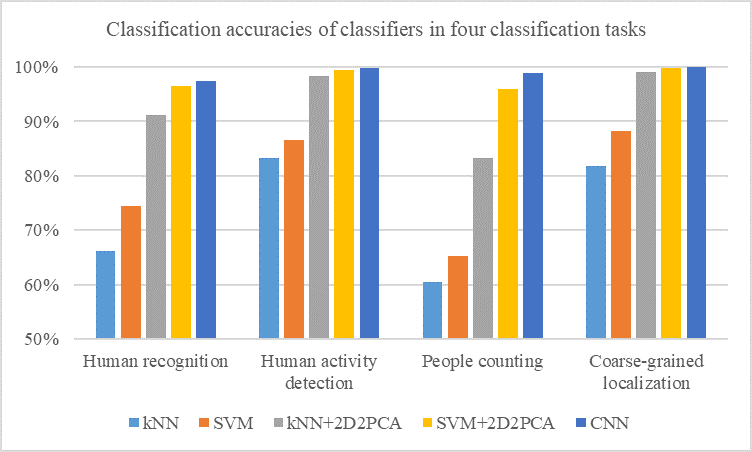
\includegraphics[width=3.6in]{result}
\caption{The performances of five classifiers in four classification tasks}
\label{fig_rsu}
\end{figure}

\begin{figure}[!t]
\centering
%\captionsetup{justification=centering}
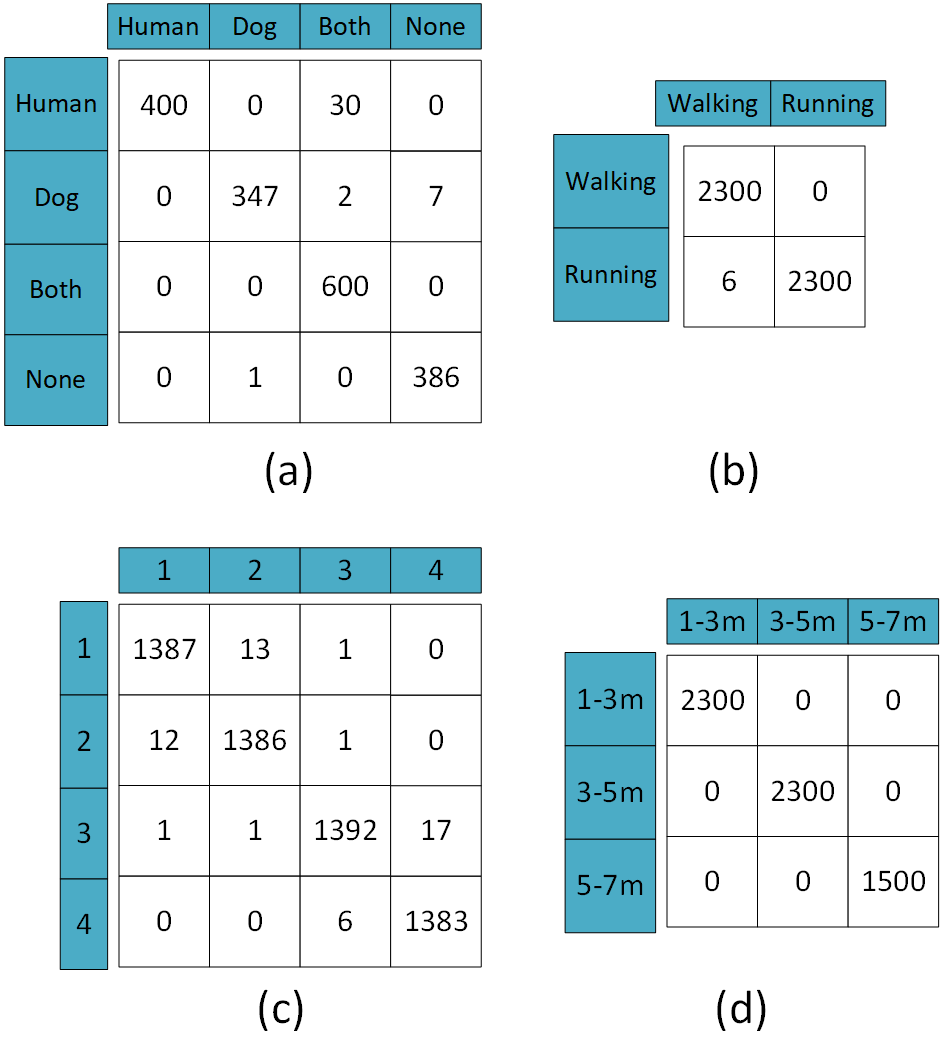
\includegraphics[width=3.4in]{confusion}
\caption{Confusion matrices of CNNs in (a). Human recognition, (b). Activity detection, (c). People counting, (d). Coarse-grained localization}
\label{fig_confusion}
\end{figure}

